\documentclass[12pt]{article}
\usepackage{tocloft}
\usepackage[polish]{babel}
\usepackage[utf8]{inputenc}
\usepackage{float}
\usepackage{enumerate}
\usepackage{listings}
\usepackage{subfig}
\usepackage{graphicx}
\usepackage{mathpazo}
\usepackage[T1]{fontenc}
\usepackage{color}
\usepackage{epstopdf}
\usepackage{amsmath, mathtools}
\usepackage{tabularx}
\usepackage[toc,page]{appendix}

\usepackage{array}
\newcolumntype{L}[1]{>{\raggedright\let\newline\\\arraybackslash\hspace{0pt}}m{#1}}
\newcolumntype{C}[1]{>{\centering\let\newline\\\arraybackslash\hspace{0pt}}m{#1}}
\newcolumntype{R}[1]{>{\raggedleft\let\newline\\\arraybackslash\hspace{0pt}}m{#1}}

\usepackage{booktabs}
\usepackage{amsfonts}
\usepackage{tikz}

\usepackage{geometry}
\geometry{verbose,tmargin=2.5 cm,bmargin=2.5 cm,lmargin=2.5 cm,rmargin=2.5 cm}

\newcommand{\code}[1]{\texttt{#1}}
\DeclareMathOperator*{\argmin}{arg\,min}

\newcommand{\bpm}{\left(\begin{matrix}}
\newcommand{\epm}{\end{matrix}\right)}
\newcommand{\grad}{\nabla}
\newcommand{\dx}{\Delta x}
\newcommand{\du}{\Delta u}
\newcommand{\dt}{\Delta t}
\newcommand{\dv}{\Delta v}
\newcommand{\dz}{\Delta z}
\newcommand{\dlam}{\Delta\lambda}
\newcommand{\dnu}{\Delta\nu}

\newcommand{\R}{\mathbb{R}}
\newcommand{\<}{\langle}
\renewcommand{\>}{\rangle}

\newcommand{\diag}{\operatorname{diag}}
\newcommand{\vzero}{\mathbf{0}}
\newcommand{\vone}{\mathbf{1}}

\usepackage[
        unicode=true,
        bookmarks=true,
        bookmarksnumbered=false,
        bookmarksopen=false,
        breaklinks=false,
        pdfborder={0 0 1},
        backref=false,
        colorlinks=false]{hyperref}
		
\hypersetup
{
        pdftitle={Rekonstrukcja obrazu z~sygnału rzadkiego},
        pdfauthor={Karol Olko, Piotr Wiśniewski}
}

\linespread{1.15}
\lstloadlanguages{TeX}

\usepackage{titlesec}
\usepackage{titletoc}

\DeclareUnicodeCharacter{00A0}{~}

\begin{document}

\author{Karol Olko, Piotr Wiśniewski}
\title{\huge{Rekonstrukcja obrazu z~sygnału rzadkiego}}
\maketitle
\newpage{}
\input{abstrakt/abstrakt}
\tableofcontents{}
\newpage{}
%%%%%%%%%%%%%%%%%%%%%%%%%%%%%%%%%%%%%%%%%%%%%%%%%%%%%%%%%%%%%%%%%%%%%%%%%
\section{Wstęp}
\subsection{Wprowadzenie}
Kierunek badań odtwarzania sygnału rzadkiego (ang. \textbf{CS} – \textit{Compressed Sensing}) jest stosunkowo nową i bardzo ciekawym kierunkiem badań w~dziedzinie przetwarzania sygnałów cyfrowych (ang. \textbf{DSP} – \textit{Digital Signal Processing}). W~klasycznym podejściu, aby dokładnie odtworzyć sygnał ciągły, próbkuje się go przynajmniej z~częstotliwością Nyquista. Dla sygnałów szybkozmiennych jest to jednak bardzo kosztowne, gdyż wymaga to znacznego skomplikowania czujników (wyposażając je w~mechanizm kompresji danych) lub wymusza wykorzystanie kanału transmisyjnego o~dużej przepustowości. Często również wykonanie samego pomiaru jest drogie i~powolne (jak w~przypadku rezonansu magnetycznego) lub niebezpieczne (promienie rentgenowskie). Wyniki badań z~dziedziny próbkowania rzadkiego dowodzą jednak, że często udaje się dokładnie odtworzyć sygnał ze znacznie mniejszej liczby pomiarów, wykorzystując jego nadmiarowość i~rzadką reprezentację w~odpowiednio dobranej przestrzeni \cite{IntroductionCS}. Ta sama idea wykorzystywana jest w~algorytmach kompresji danych: rzadka reprezentacja zdjęcia w~bazie falkowej jest metodą zmniejszenia wielkości obrazu w~standardzie JPEG2000 \cite{JPEG2000}. Algorytmy CS są zasadniczo różne - próbują one znaleźć taki sposób pomiaru, który pobiera konieczne informacje o~sygnale już w~skompresowanej formie. Proces odtwarzania sygnału możemy więc podzielić na dwie podstawowe czynności - rzadkie próbkowanie i~rekonstrukcję. Drugi krok jest nietrywialny i~kosztowny pod względem obliczeniowym. Zazwyczaj zadanie rekonstrukcji sygnału sprowadza się do liniowego lub kwadratowego problemu optymalizacji, w~którym najwięcej czasu zajmuje obliczenie kroku Newtona \cite{L1MagicNotes}.

\subsection{Cele i~założenia projektu}
Głównym celem projektu była implementacja wybranego algorytmu odtwarzania sygnału rzadkiego, wykorzystując do obliczeń kartę graficzną. Zadaniem dodatkowym była symulacja jednopikselowej kamery, wykorzystując kamerę firmy Jai, dostępną w~sali laboratoryjnej. Projekt miał umożliwić znaczne przyspieszenie istniejących rozwiązań, opartych głównie o~skrypty środowiska Matlab/Simulink, a~także umożliwić odtwarzanie obrazów o~większej skali (docelowo obraz w~pełnej rozdzielczości kamery, czyli 2560 x 2048 pikseli). Z~uwagi na przyjęty sposób uzyskiwania pomiarów oraz przede wszystkim - ograniczenia pamięciowe, okazało się to kompletnie nierealne. Projekt zrealizowano w~znacznie mniejszej skali, dając jednak możliwość na jego dalszą rozbudowę (co, według naszej wiedzy, byłoby możliwe przy innym sformułowaniu problemu).

\subsubsection{Budowa jednopikselowej kamery}
Pierwszym krokiem w~realizacji projektu było dokładne zaznajomienie się z~urządzeniem, którego działanie mieliśmy symulować. Pomogło nam to zrozumieć praktyczny kontekst przy zapoznawaniu się z~publikacjami naukowymi oraz poznać ograniczenia przy projektowaniu algorytmów odtwarzania obrazu narzucone przez sprzęt.

\begin{figure}
\centering
	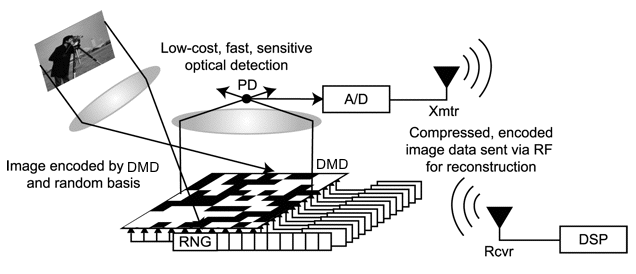
\includegraphics[width=\textwidth]{rysunki/cscam.png}
\caption{Schemat jednopikselowej kamery}
\label{fig:singlePixelSchema}
\end{figure}

\begin{figure}
\centering
	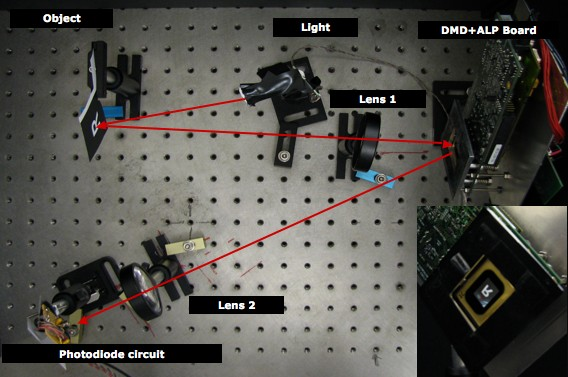
\includegraphics[width=0.6\textwidth]{rysunki/cscamerasetup.jpg}
\caption{Zestawienie jednopikselowej kamery na stanowisku laboratoryjnym}
\label{fig:singlePixelSetup}
\end{figure}

Jednopikselowa kamera to prototyp urządzenia pomiarowego, skonstruowany przez naukowców uniwersytetu RICE \cite{SinglePixelCamera}. Składa się ona z~jednej fotodiody ("piksela"), dwóch soczewek i~matrycy mikroluster (ang. \textbf{DMD} - \textit{Digital Micromirror Device}) \ref{fig:singlePixelSetup}. Ustawienie luster macierzy jest sterowane komputerowo. Podanie 1 na poszczególny element DMD powoduje jego skierowanie w~kierunku drugiej soczewki, zaś 0 - z~dala od niej. Wartości między 0 a~1 mogą być uzyskane przez wielokrotne sterowanie elementem matrycy w~czasie całkowania sygnału na odbiorniku. Zgromadzone na fotodiodzie napięcie jest konwertowane do postaci cyfrowej i~wysyłane drogą radiową do odbiornika \ref{fig:singlePixelSchema}. Ze względu na długi proces pomiarowy, trudno wyobrazić sobie, by powyższa konstrukcja była w~stanie wyprzeć zwykłe kamery w~codziennych zastosowaniach. Może jednak stanowić atrakcyjną cenowo alternatywę dla czujników światła w~zakresach niewidzialnych dla oka.

\subsubsection{Formalne sformułowanie problemu}
W swym doskonałym artykule \cite{CandesIntro} Emmanuel Candes, jeden z~pionierów dziedziny przetwarzania rzadkiego, przedstawił podstawowe obserwacje naukowców umożliwiające zastosowanie metody, dokonał pewnych oszacowań ilościowych, dotyczących potrzebnej liczby pomiarów i~ograniczeń metody na dzisiejszym etapie rozwoju.
Dziedzina przetwarzania rzadkiego wykorzystuje fakt \textit{rzadkości} sygnału oraz \textit{niekoherencji} \cite{Candes2006} różnych baz przestrzeni liniowych. Pierwsze z~pojęć oznacza możliwość przechowania większości użytecznych informacji o~sygnale w~niewielkim obszarze danych. Ściślej rzecz biorąc, reprezentacja $x = \phi \alpha$ w~bazie $\phi$ jest k-rzadka, gdy $K \ll N$ współczynników $\alpha$ dokładnie opisuje $x$. Niekoherencja wyraża z~kolei ideę, że mając rzadką reprezentację sygnału w~jednej bazie, jest ona znacznie rozłożona w~innej. Przykładem może być delta Diraca, która choć w~dziedzinie jest reprezentowana przez jeden pik, jest funkcją stałą w~całej dziedzinie częstotliwości. Wykorzystując dwie powyższe obserwacje, można skonstruować taki sposób pomiaru, który próbkuje go od razu w~skompresowanej formie, bez potrzeby jego zrozumienia. 

Przyjmujemy, że informacja o~sygnale $f_t$ jest uzyskiwana poprzez liniowe funkcjonały
\begin{equation}
	y_k = <f, \varphi_k>, k = 1,...,m.
\end{equation}
Gdzie $\varphi_k$ wyraża sposób pomiaru. Przykładowo, dla matrycy CCD będzie to funkcja charakterystyczna jej danego piksela, a~dla rezonansu magnetycznego - sinusoida o~określonej częstotliwości.

Sposób wykonania m pomiarów przechowujemy w~macierzy pomiarowej $A \in R^{M*N}$. Tym samym, problem CS może zostać opisany jako nieoznaczone równanie liniowe: 
\begin{equation}
	y = A \cdot x
	\label{eq:lin}
\end{equation}

Powyższe równanie posiada nieskończoną liczbę rozwiązań z~$N - M$ stopniami swobody. Rekonstrukcja $x$ polega na takim wybraniu rozwiązania, które najlepiej spełnia postawione przed nim dodatkowe założenia. Najbardziej oczywistym jest znaleźć najrzadsze rozwiązanie, tzn.
\begin{equation}
	\hat{x} = \argmin_z \|x_0\| \text{spełniający} \Phi x=y
	\label{eq:l0}
\end{equation} \cite{CandesIntro, Davenport2010, Zhang2013}, gdzie $\|x\|_0$ = ilość niezerowych współczynników x. Użycie normy zero cechuje się jednak kombinatoryczną złożonością obliczeniową i nie jest realizowalne w dużej skali. Najczęściej jednak udaje się dokładnie odzyskać rzadki sygnał, rozwiązując problem prostego dopasowania (\textbf{BP} - \textit{basis pursuit}):
\begin{equation}
\min_{x \in R^n} \|x_1\| 
\label{eq:l1}
\end{equation}, gdzie $\|x\|_1 = \sum_{i=1}^{n} |x_i|$. Problem \ref{eq:l1} ma wyraźną przewagę nad \ref{eq:l0}, gdyż daje się rozwiązać metodami programowania liniowego \cite{Fountoulakis2012}. Część algorytmów odtwarzania sygnałów rozwiązuje zmodyfikowaną wersję \ref{eq:l1}. Istnieje również wiele metod rekonstrukcji sygnału, wykorzystując algorytmy zachłanne, stochastyczne lub wariacyjne.
 
Warto przy tej okazji wspomnieć, że przetwarzanie rzadkie wykorzystywane jest także dla sygnałów ciągłych \cite{Eldar2009}, zaszumionych i~nie całkowicie rzadkich \cite{Cevher2009}. W~takim wypadku $\alpha$ stanowi aproksymację $x$. Jak pokazują wyniki rekonstrukcji zdjęć, są one wciąż bardzo skuteczne. 
\newline{}
Istotnym osiągnięciem CS jest jego zdolność do oszacowania liczby pomiarów tak, by rekonstrukcja przebiegła pomyślnie z~prawdopodobieństwem bliskim pewności \cite{CandesIntro}. Jest ona zależna od rzadkości reprezentacji sygnału w~danej bazie oraz niekoherencji bazy, w~której próbkujemy sygnał z~bazą rozrzedzającą $x$. Wielkość tę definiujemy następująco:
\begin{equation}
	\mu (\Phi,\Psi) = \sqrt{n} \max_{i, j} |<\phi_i, \psi_j>|
	\label{eq:coherence}
\end{equation}
Okazuje się, że bezpiecznym wyborem jest losowe próbkowanie sygnału, gdyż jest ono niekoherentne z~dowolną, ustaloną bazą $\phi$. Pozostaje więc odpowiednio dobrać sposób jego reprezentacji.

\subsection{Zarys proponowanego rozwiązania}
Rozwiązanie problemu CS wymaga podjęcia kilku kluczowych decyzji. Po pierwsze, należy starannie wybrać sposób próbkowania sygnału, bazę, w~której będzie on reprezentowany oraz algorytm jego rekonstrukcji. W~rozważaniach należy również wziąć pod uwagę docelową architekturę sprzętową i~jej możliwie pełne wykorzystanie.
\subsubsection{Wybór macierzy pomiarowej}
Punktem wyjścia w~badaniach był pakiet $\ell_1$-magic \cite{SinglePixelCameraCode}, zawierający kod źródłowy wybranych algorytmów odtwarzania sygnałów oraz dokument \cite{L1MagicNotes}  je opisujący. Pierwszym ważnym wnioskiem płynącym z~publikacji jest konieczność wyrażenia macierzy pomiarowej w~sposób ukryty, nie wymagający jawnego przechowywania w~pamięci. Jej wielkość bardzo szybko urasta bowiem do ogromnych rozmiarów. Dla przykładu, macierz pomiarowa eksperymentu, w~którym dokonano 20 \% pomiarów zdjęcia o~wielkości 256x256 pikseli, zapisana w~formacie \textit{float} będzie zajmować ponad 3GB pamięci, stanowczo za dużo, zmieścić ją w~RAM GPU.~Powyższy wniosek stanowi to problem z~dwóch powodów. Po pierwsze, jak w~skompresowany sposób zapisać losowe ciągi liczb wysyłane do DMD? Po drugie, zastosowanie implikowanej formy macierzy znacznie utrudnia przyspieszenie obliczeń za pomocą karty graficznej. Nie próbując jednak od razu odpowiedzieć na wszystkie stawiane wyzwania, rozpoczęto badania bogatej literatury CS.~We wstępie \cite{Fountoulakis2012} dostępny jest imponujący przegląd dostępnych metod próbkowania i~odzyskiwania sygnału. Oprócz braku konieczności przechowywania macierzy pomiarowej w~pamięci, autor narzuca ciekawe ograniczenie - możliwie szybkie mnożenie macierzy z~wektorem (np. $\mathcal{O}(nlog(n))$ lub $\mathcal{O}(n)$).  Przyspieszenie tej operacji znacząco skróci czas odtwarzania sygnału, bez względu na wykorzystaną architekturę sprzętową. 
\newline{}
Ciekawą propozycją autorów jest niepełna macierz Fouriera. Jej konstrukcja polega na losowym wybraniu m rzędów macierzy Fouriera o~rozmiarze n x n. Nie wymaga przechowywania w~pamięci, a~jej iloczyn z~wektorem daje się szybko obliczyć wykorzystując algorytm FFT (cechuje się on złożonością $\mathcal{O}(nlog(n))$). Niestety, jej postać spełnia \ref{eq:l1} z~ogromnym prawdopodobieństwem dla znacznie większej liczby pomiarów niż wykorzystując zwykłą macierz losową o~rozkładzie Gaussa  \cite{Rudelson2008}. Postanowiono więc poszukać innych rozwiązań. W~swym doskonałym artykule \cite{Peyre2010}, Gabriel Peyre ocenia kilka ortonormalnych baz, które mogą posłużyć jako sposoby rzadkiej reprezentacji sygnału. W~praktyce zdjęcia są skutecznie rozrzedzane przez bazę falkową, kosinusową czy curvelet \cite{CurveletWebSite, Candes2000}. Według autora, każda z~powyższych posiada swe wady i~zalety, zatem aby móc odtwarzać sygnał o~różnej charakterystyce, bazę reprezentacji należy dobierać dynamicznie. Jest to niewątpliwie ciekawe podejście, ale wymagające ogromnego nakładu pracy i~zostało porzucone. Z~tego samego powodu porzucono również ideę poszukiwania najrzadszej bazy sygnału poprzez estymację macierzy $Q$ transformacji Karhunena-Loeve'a \cite{Gwon2012}. \footnote{Odzyskujemy $s = Q^H x$, gdzie $R_x = E[xx^H]$ i~$R_x = Q \Lambda Q^H$. Kolumny $Q$ to wektory własne $R_x$, $\Lambda$ to diagonalna macierz wartości własnych.} Zainteresowało nas jednak próbkowanie sygnału za pomocą podmacierzy bazy Hadamarda-Walsha. Jej definicja jest prosta \footnote{$W_0$ = 1, $W_j = \frac{1}{\sqrt{2}} \begin{Bmatrix} W_{j-1} & W_{j-1} \\ W_{j-1} & -W_{j-1} \end{Bmatrix}$}, a~będąc mocno związaną z~bazą Fouriera, pozwala na mnożenie wektorów ze złożonością $\mathcal{O}(nlog(n))$. Ten sam pomysł, choć w~bardziej przejrzysty sposób, przedstawiono również w~\cite{Davenport2010} i~w~ramach praktycznego przykładu odniesiono go do jednopikselowej kamery. Macierz pomiarową możemy generować poprzez 
\begin{equation}
	\Phi = \left(\frac{1}{2} \sqrt{N} I_\Gamma W_B + \frac{1}{2} \right) D
\end{equation}
Gdzie $I_\Gamma$ oznacza identycznościową podmacierz $M x N$, uzyskaną przez losowy wybór $M$ wierszy, tak, by $I_\Gamma W_B$ była podmacierzą $W_B$ indeksowaną przez $\Gamma$. Ponadto, $D$ oznacza losową macierz permutacji o~rozmiarze $N x N$. Wyrażenie $\frac{1}{2} \sqrt{N} I_\Gamma W_B + \frac{1}{2}$ przeskalowuje elementy macierzy $\Phi$ tak, by mieściły się w~zakresie $(0,1)$. Metoda generowania pomiarów wygląda na bardzo atrakcyjną. Niestety, algorytm szybkiego mnożenia macierzy $W_B$ istnieje tylko dla rozmiarów $2^N$. Ponadto, wynik pomiarów sygnału wyrażonego w~bazie falkowej $\Phi \Psi$ nie daje teoretycznych gwarancji odtworzenia $x$ z~ogromnym prawdopodobieństwem (choć przedstawiona metoda w~praktyce daje dobre, powtarzalne rezultaty). Z~tego powodu postanowiono poszukać innego rozwiązania. W~ciekawym artykule naukowców z~uniwersytetu RICE \cite{Baraniuk2010} opisano możliwość założenia pewnej struktury sygnału, co ogranicza przestrzeń rozwiązań, a~co za tym idzie - zmniejsza liczbę potrzebnych pomiarów i~złożoność obliczeniową algorytmów. Dodatkowo, posiadanie pewnych założeń co do odzyskiwanych danych ułatwia rozróżnienie ich od szumu, co zwiększa stabilność procesu. Niestety, autorzy pracy nie zaproponowali takiego rozwiązania, które z~jednej strony znacznie ułatwiałaby odzyskanie sygnału, a~z~drugiej - było dostatecznie elastyczne. 

Ostatecznie, naszym wyborem stała się rzadka macierz pomiarowa, opisana w~\cite{Berinde2008}. Cechuje ją niezwykła prostota. W~każdej kolumnie macierzy $A$ wybieramy $d$ jedynek. Dbamy przy tym, by żadne dwa wektory kolumnowe nie były identyczne (co przy $d \ll N$ jest praktycznie niemożliwe). Zaletą tego rozwiązania jest udowodniona odporność na szum, efektywne mnożenie macierzy (wymaga ono nie więcej niż $nd$ dodawań) i~niewielka ilość zajmowanego miejsca w~pamięci. Przedstawione wyniki empiryczne dla zdjęć o~rozmiarze 256x256 potwierdziły, że wykorzystując tę macierz pomiarową, można rozwiązywać problemy w~odpowiednio dużej skali. Po decyzji związanej z~macierzą pomiarową, przystąpiono do wyboru algorytmu rekonstrukcji zdjęcia.

\subsubsection{Dobór algorytmu rekonstrukcyjnego}
Odpowiedni dobór algorytmu odtworzenia sygnału ma niebagatelne znaczenie na szybkość, stabilność i~dokładność procesu. Wyzwaniem stało się odpowiednie dobranie metody dla implementacji na karcie graficznej. Temat ten jest bowiem rzadko podejmowany w~publikacjach naukowych. Natrafiono jedynie na jedną bibliotekę implementującą algorytmy odtwarzania sygnału z~użyciem kart graficznych \cite{GAGA}, zbudowaną na bazie biblioteki CUDA \cite{CUDA}. Grupa metod optymalizacji tam wykorzystanych nosi miano zachłannych. Natrafiono na doskonałe przeglądy metod z~tego obszaru w~\cite{Needell2009,Gronde2008}. Przykładowo, przedstawiony tam algorytm iteracyjnego progowania (ang. \textbf{IHT} -- \textit{Iterative hard thresholding}) \cite{Blumensath2009} opisany jest następującą, iteracyjną formułą: 
\begin{equation}
\begin{split}
    x_0 & = 0 \\ 
x_{n+1} & = H_s \left(x_n + \Phi^T(y - \Phi x_n) \right)
\end{split}
\end{equation}
\newline{}
Gdzie $H_s(a)$ zeruje wszystkie poza $s$ największymi współczynniki $x$. Algorytm cechuje niezwykła prostota. Jedna jego iteracja wymaga dwóch mnożeń macierz-wektor i~częściowego posortowania elementów $a_n =  H_s \left(x_n + \Phi^T(y - \Phi x_n) \right)$. Łatwo wyobrazić sobie równoległą implementację takiego rozwiązania, np. przy użyciu algorytmu \textit{mergesort} \cite{Thouti2012}. Dodatkową zaletą rozwiązania jest niewielka ilość przechowywanych danych. Niestety, prostota i~szybkość algorytmu odbija się na jego dokładności. W~kontekście zdjęć ich wyjście może stanowić pierwsze przybliżenie rozwiązania problemu \ref{eq:l1}. W~szczególności, metody zachłanne słabo aproksymują niezbyt rzadki sygnał ($\frac{k}{n} \ge 0.2$, gdzie $k$ - liczba znaczących elementów $x$, $n$ - rozmiar $x$). Z~tego powodu zrezygnowano z~tej klasy algorytmów i~zwrócono się w~stronę klasycznych metod optymalizacyjnych rozwiązujących problem \ref{eq:l1} lub pokrewny.

Ponownie, punktem wyjścia w~naszych rozważaniach były algorytmy zaimplementowane w~pakiecie $\ell 1$-MAGIC \cite{SinglePixelCameraCode}. Grupa metod programowania liniowego minimalizujących normę $\ell 1$ okazały się jednak skutecznie głównie dla sygnałów prawdziwie rzadkich. Odtworzenie zdjęcia algorytmem $\ell 1$-pd \cite{Boyd2004} w~aplikacji współtworzonej przez jednego autorów projektu \cite{PR12SIS306} było skuteczne, gdy $\frac{m}{n} \ge  0.6$. Chcąc znacząco poprawić ten wynik, należało poszukać innej metody rozwiązania. Pamiętając również o~akceleracji obliczeń przy pomocy karty graficznej, przyglądnięto się klasie algorytmów zwykle implementowanych na tych urządzeniach. 

Za niezwykle interesujący uznano algorytm \textbf{TVQC} \cite{Candes2005a,Candes2005b}. Traktując $x_{ij}$ jako piksel znajdujący się w~$i$-tym rzędzie oraz $j$-tej kolumnie zdjęcia $x$ o~wymiarach $n \times n$, oraz po zdefiniowaniu operatorów:
\begin{equation}
	D_{h;i,j}x = \begin{cases}
					x_{i+1,j} - x_{i,j} &, i < n \\
					0 &, i = n 
				 \end{cases} 
				 \qquad
	D_{v;i,j}x = \begin{cases}
					x_{i,j+1} - x_{i,j} &, j < n \\
					0 &, j = n
				 \end{cases}			 
\end{equation}
Algorytm ten można opisać jako rozwiązanie następującego problemu optymalizacyjnego:
\begin{equation}
\begin{split}
& \min_{TV} ~~\text{spełniający}~~\|Ax - y \|_{\ell 2} \le \epsilon \\
\text{gdzie:} &\\
              & \|x \|_{TV} = \sum_{i,j} \sqrt{ \left( D_{h;i,j} \right)^2 + \left( D_{v;i,j} \right) ^2} = \sum_{i,j}|\left(D_{i,j}\right) |
\label{eq:TV}
\end{split}
\end{equation}

Podstawowym założeniem tej metody jest rzadkość (lub kompresowalność) \textit{gradientu} zdjęcia. Jest ono słuszne dla dużej części naturalnych ekspozycji i~tylko nieznacznie zmniejsza uniwersalność metody. Baza gradientu sygnału wydaje się być wysoce niekoherentna z~rzadką macierzą pomiarową. Dokonano bowiem udanych rekonstrukcji zdjęć przy użyciu ok. 8\% pomiarów \cite{Berinde2008}. Jedyną zagadką pozostała ocena wydajności algorytmu zaimplementowanego na karcie graficznej. Nie odnaleziono bowiem żadnych prób równoległej implementacji algorytmu. Ustalono jednak\cite{Tarsa2012, Bolz2003}, że możliwe jest wyraźne przyspieszenie najbardziej kosztownego etapu algorytmu - obliczenie kroku Newtona przy pomocy iteracyjnej metody gradientu sprzężonego. Po długich rozważaniach przyjęto w~końcu sposób realizacji algorytmu i~przystąpiono do oceny jego złożoności obliczeniowej oraz możliwości stanowiska laboratoryjnego. Miało to bezpośrednie przełożenie na skalę rozwiązywanych później problemów.

\subsection{Omówienie zawartości pracy}
Poniższy raport składa się z~sześciu rozdziałów. Po wstępie, w~którym opisano kontekst pracy i~wykonane badania literaturowe, następuje rozdział poświęcony złożoności czasowej i~pamięciowej postawionego problemu. Rozdział trzeci przedstawia koncepcję jego rozwiązania, a~czwarty - procedury testowe. Rozdziały 5 i~6 opisują odpowiednio wyniki przeprowadzonych eksperymentów oraz podsumowanie. Szczegółowy opis zadania znajduje się w~załączniku.

\newpage{}
\section{Analiza złożoności i estymacja zapotrzebowania na zasoby}
Pierwszym i niezbędnym krokiem przy pracy na stanowisku laboratoryjnym było zapoznanie się z dostępną architekturą sprzętową oraz wybór środowiska programistycznego. Następnie, zapoznano się i opisano standard OpenCL, w ramach którego implementowano algorytm rekonstrukcji obrazu na kartach graficznych. Należało bowiem poznać szczególne wymagania oraz ograniczenia wynikające z jego użycia. Dalszą część rozdziału stanowi oszacowanie złożoności pamięciowej i obliczeniowej wybranego algorytmu odtwarzania obrazu.
\subsection{Sprzęt uruchomieniowy}
Dostępny w laboratorium komputer składał się z wielordzeniowego procesora klasy Intel i5 oraz dwóch kart graficznych firmy Nvidia GeForce GTX670. W poniższej tabeli zebrano ich główne parametry:

\begin{table}[H]
\begin{center}
\begin{tabular}{|c|c|}
\hline
         & Nvidia GeForce GTX 670  \\
\hline
        Liczba rdzeni & 1344 \\
\hline
        Częstotliwość bazowa & 915 [MHz] \\
\hline
        Pojemność pamięci & 2048 [MB] \\
\hline
        Magistrala & 256 [bit] \\
\hline
\end{tabular} 
\caption{Wybrane parametry kart graficznych Nvidia GTX 670}
\label{tab:PGU}
\end{center}
\end{table}

Liczba rdzeni wykorzystywanej przez nas karty graficznej jest wprost imponująca. Potencjalnie, wykorzystanie tej ilości jednostek obliczeniowych może dać kolosalne korzyści czasowe. Program, który w skuteczny sposób wykorzystuje powyższe zasoby, musi dokonać kilku niskopoziomowych optymalizacji. Doskonałą lekturę w tym zakresie stanowiła książka opisująca bibliotekę OpenCL \cite{Scarpino2012}. Po pierwsze, należy minimalizować liczbę rozgałęzień algorytmu. Po drugie, zadania na karcie graficznej należy dzielić tak, by zależności między wątkami były jak najmniejsze - konieczność synchronizacji znacznie zmniejsza wydajność programu. Po trzecie, należy minimalizować liczbę odwołań wątków karty graficznej do pamięci globalnej - podręczne zasoby lokalne charakteryzują się znacznie mniejszym opóźnieniem. W końcu, należy liczyć się z każdorazowym opóźnieniem obliczeń na GPU, ze względu na dwukrotny transfer danych między hostem a urządzeniem.

Zdecydowano się na implementację programu w języku C++, z wykorzystaniem środowiska Visual Studio. Wynikało to z kilku przyczyn. Po pierwsze, wybór był konsekwencją doświadczenia zawodowego autora. Pisanie kodu w znanym sobie języku i środowisku znacznie przyspieszyło pracę. Po drugie, przygotowany SDK kamery Jai zawierał binding w tym właśnie języku, co znacznie uprościło integrację tego modułu programu. C++ pozwolił twórcom z jednej strony zdekomponować problem obiektowo, a z drugiej - skompilować program natywnie, licząc na optymalną wydajność. Z perspektywy czasu trzeba jednak rozważyć, czy nie lepiej wykorzystać Pythona, z uwagi na duże wsparcie biblioteczne tego języka, a także czytelność i zwartość kodu. Ostatecznym celem programu było bowiem maksymalne wykorzystanie karty graficznej, z minimalną ingerencją komputera-hosta. Ponadto, krytyczne dla wydajności procedury można by zawrzeć w formie skompilowanej biblioteki języka C. Ciekawym byłoby zatem porównać nakład pracy przygotowanych programów i ich wydajność.

\subsection{Standard OpenCL}
Jednym z głównym wyzwań projektu było zaznajomienie się i wykorzystanie standardu OpenCL \cite{OpenCL} do programowania w heterogenicznym środowisku obliczeniowym. W przeciwieństwie do rozwijanego przez firmę Nvidia standardu CUDA, OpenCL może być wykorzystywany na różnych platformach sprzętowych, o ile tylko standard jest wspierany przez producenta. Choć OpenCL definiowuje tylko interfejs programistyczny w języku C oraz wrapper w C++, dostępne są również jego realizacje w Javie, Pythonie i innych. W chwili pisania raportu, opublikowano wersję 2.0 tego dokumentu. Niestety, żaden z producentów kart graficznych jeszcze go nie wspiera. Posługiwano się więc interfejsem programistycznym standardu w wersji 1.2.

Na podstawowe pojęcia w OpenCL składają się: \textit{host} i \textit{device}, na których wykonywana jest aplikacja. \textit{Host} to zwykle CPU, wysyłające rozkazy do GPU (\textit{device}), w szczególności w celu wykonywania \textit{kerneli}, czyli dynamicznie kompilowanych programów. Pojedynczy rdzeń procesora karty graficznej zwany jest \textit{work-itemem}. Pewien zbiór tychże stanowi \textit{work-group}. Jednostki obliczeniowe rozróżniane są globalnym identyfikatorem \textit{globalID}, a grupy - \textit{localID}. 
Pamięć \textit{device} możemy podzielić na 4 typy: private, local, constant, global. Ich dostęp możliwy jest odpowiednio: \textit{work-item}, \textit{work-group} oraz cały \textit{device}. Cechują się one kolejno rosnącą pojemnością. Niestety, wielkość pamięci idzie w parze z coraz dłuższym czasem dostępu.

\subsection{Wykorzystanie biblioteki ViennaCL w projekcie}
Pokrótce analizując kod źródłowy pakietu $\ell_1$-MAGIC, szybko zrozumiano, że napisanie i przetestowanie \textit{kerneli} dla karty graficznej będzie zadaniem karkołomnym. Standard w swej naturze jest bardzo niskopoziomowy, co z jednej strony zapewnia elastyczność - ale z drugiej, niską efektywność pracy. Zdolność do debugowania kodu przeznaczonego na kartę graficzną jest ograniczona. W dodatku, współbieżna praca wielu wątków programu jest częstym błędem występowania trudnych w zreprodukowaniu i zrozumieniu błędów. Z tego powodu zdecydowano się wykorzystać bibliotekę \textbf{ViennaCL} \cite{ViennaCL}, która oferuje wysokopoziomowy interfejs programistyczny do przygotowania i uruchamiania zadań na karcie graficznej, zawiera wiele przydatnych, gotowych funkcji, takich jak solvery układów liniowych, metody dekompozycji macierzy, a w końcu - jest niezwykle elastyczna, pozwalając na uruchamianie własnoręcznie napisanych \textit{kerneli}.

\subsection{Oszacowanie złożoności algorytmu TVQC}

\newpage{}
\section{Koncepcja proponowanego rozwiązania}
Jednym z głównych celów przyświecających autorowi programu było stworzenie jasnej, przejrzystej i modularnej struktury aplikacji, umożliwiającej łatwą analizę funkcjonalną i późniejszą możliwość rozszerzeń. Zdefiniowano zatem szereg interfejsów, które są jego "stopniami swobody". Poniżej przedstawiono diagramy klas, zależności między nimi oraz ich wykorzystanie w trakcie działania programu.
\subsection{Interfejsy programu}
\subsubsection{Interfejs macierzy}
(...)
\subsubsection{Interfejs kamery}
(...)
\subsubsection{Interfejs Solvera}
(...)
\subsubsection{Interfejs Algorytmu}
(...)
\subsection{Działanie aplikacji}


\newpage{}
\input{testowanie/testowanie}
\section{Rezultaty i wnioski}
(...)
\input{podsumowanie/podsumowanie}

%%%%%%%%%%%%%%%%%%%%%%%%%%%%%%%%%%%%%%%%%%%%%%%%%%%%%%%%%%%%%%%%%%%%%%%%%

\cleardoublepage

\listoffigures{}

\newpage{}

\nocite{*}
\bibliographystyle{plain}
\bibliography{bibliografia}

\begin{appendices}
\section{Szczegółowy opis zadania}
\subsection{Specyfikacja projektu}
Celem projektu było zaproponowanie realistycznego modelu jednopikselowej kamery oraz przygotowanie co najmniej jednej metody odtwarzania rzadko spróbkowanego sygnału. Zadanie to wydaje się mieć wiele potencjalnych zastosowań, szczególnie w dziedzinie medycyny lub telekomunikacji. Oczekiwanym celem projektu jest maksymalne przyspieszenie działania algorytmu, poprzez wykorzystanie zasobów karty graficznej. 
\subsection{Szczegółowy opis algorytmu odtwarzania obrazu TVQC}
Algorytm TVQC został dokładnie zdefiniowany w dokumentacji pakietu $\ell_1$-MAGIC ~\cite{L1MagicNotes}. Metoda optymalizacji wykorzystana do odtworzenia zdjęcia została z kolei opisana w \cite{Boyd2004}. Poza przepisem matematycznym, przedstawiono również funkcjonowanie algorytmu na schemacie blokowym.
\subsubsection{Zdefiniowanie problemu}
Algorytm TVQC należy do grupy kwadratowych problemów optymalizacji (ang. \textbf{SOCP} - \textit{Second-order Cone Programming}). Przepiszmy więc problem ~\ref{eq:TV} do ich generycznej postaci:

\begin{equation}
\begin{split}
\min_{x,t} \sum_{ij} t_{i,j} \text{~~spełniający~~} &\|D_{ij}x \|_2 < t_{ij}, i,j = 1,...,n \\
&\|Ax - b \|_2 \le \epsilon.
\end{split}
\label{eq:SOCP-generic}
\end{equation}
Przyjmując
\begin{equation}
\label{eq:ftij}
f_{t_{ij}} = \frac{1}{2}\left(\|D_{ij}\|_2^2 - t^2_{ij}\right)\quad i,j=1,\ldots,n
\end{equation}
oraz
\[
f_\epsilon = \frac{1}{2}\left( \|Ax-b\|^2_2 - \epsilon^2\right),
\].
Mając
\[
\grad f_\epsilon = \bpm A^Tr \\ \vzero \epm,\quad 
\grad f_\epsilon \grad f_\epsilon^T =
\bpm  A^Trr^TA & \vzero \\ \vzero & \vzero \epm, \quad
\grad^2 f_\epsilon = \bpm A^*A & \vzero \\
\vzero & \vzero \epm
\]
gdzie $r = Ax - b$.
Także, 
\[
\grad^2 f_{t_{ij}} = \left(\begin{array}{cc} D_{ij}^*D_{ij} & \vzero \\
\vzero & -\delta_{ij}\delta_{ij}^T \end{array}\right)
\quad
\grad^2 f_\epsilon = \left(\begin{array}{cc} A^*A & \vzero \\
\vzero & \vzero \end{array}\right).
\]

Rozważana forma kwadratowa przedstawia się następująco:
\[ 
\bpm H_{11} & B\Sigma_{12} \\
\Sigma_{12}B^T & \Sigma_{22} \epm
\bpm \dx \\ \dt \epm =
\bpm D_h^T F_t^{-1}D_h x + D_v^TF_t^{-1}D_v x + f_\epsilon^{-1}A^Tr \\
-\tau\mathbf{1} - tf^{-1}_t \epm :=
\bpm w_1 \\ w_2 \epm.
\]
gdzie $(tf^{-1}_t)_{ij} = t_{ij}/f_{t_{ij}}$, oraz 
\begin{align*}
H_{11} = ~& D_h^T(-F_t^{-1})D_h ~+~ D_v^T(-F_t^{-1})D_v ~+~ B F_t^{-2}B^T ~- \\
 & f_\epsilon^{-1} A^TA ~+~ f_\epsilon^{-2} A^Trr^TA, \\
\Sigma_{12} = ~& -TF_t^{-2}, \\
\Sigma_{22} = ~& F_t^{-1} + F_t^{-2}T^2,
\end{align*}
Rugując $\dt$
\[
\dt = \Sigma_{22}^{-1}(w_2 - \Sigma_{12}\Sigma_{\partial h}D_h\dx - \Sigma_{12}\Sigma_{\partial v}D_v\dx),
\]
kluczową do rozwiązania formą kwadratową jest
\[
H'_{11}\dx  = 
w_1 - (D_h^T\Sigma_{\partial h} + D_v^T\Sigma_{\partial v} )\Sigma_{12}\Sigma_{22}^{-1}w_2
\]
gdzie
\begin{align*}
H'_{11} = ~& H_{11} - B\Sigma^2_{12}\Sigma_{22}^{-1}B^T \\
= ~& D_h^T(\Sigma_b\Sigma^2_{\partial h}-F_t^{-1})D_h ~+~
D_v^T(\Sigma_b\Sigma^2_{\partial v}-F_t^{-1})D_v ~+~\\
~& D_h^T(\Sigma_b\Sigma_{\partial h}\Sigma_{\partial v})D_v ~+~
D_v^T(\Sigma_b\Sigma_{\partial h}\Sigma_{\partial v})D_h ~-~ \\
~& f_\epsilon^{-1} A^TA ~+~ f_\epsilon^{-2} A^Trr^TA, \\
\Sigma_b = ~& F_t^{-2} - \Sigma_{12}^2\Sigma_{22}^{-1}.
\end{align*}

Powyższy układ równań jest dodatnio określony, co pozwala rozwiązać go metodą gradientu sprzężonego.

W celu rozwiązania powyższego problemu użyto metody \textit{log-barrier} \cite{Boyd2004}. Przekształca ona \textit{SOCP} w szereg problemów z ograniczeniami liniowymi:
\begin{equation}
\label{eq:logbarrier} 
\min_z ~ \<c_0,z\> + \frac{1}{\tau^k} \sum_{i}
-\log(-f_i(z)) \quad\text{spełniający}\quad A_0 z=b,
\end{equation}
gdzie $\tau^k > \tau^{k-1}$. Ograniczenia nierównościowe zostały włączone do funkcjonału w postaci \textit{funkcji kary} (wybór $-\log(-x)$ dla funkcji bariery nie jest przypadkowy, gdyż posiada ona pożądaną własność (samozgodność \footnote{$|f'''(x)| \le 2f''(x)^{3/2}$}), która ułatwia szybką zbieżność \eqref{eq:logbarrier} do \eqref{eq:SOCP-generic} zarówno w teorii, jak i praktyce), która jest nieskończona gdy ograniczenie jest przekroczone i gładka na pozostałym obszarze.   Gdy $\tau^k$ rośnie, rozwiązanie $z^k$ problemu \eqref{eq:logbarrier} zmierza do rozwiązania $z^\star$  \eqref{eq:SOCP-generic}: 
Można wykazać, że $\<c_0,z^k\> - \<c_0,z^\star\> < m/\tau^k$, tzn. znajdujemy się o mniej niż $m/\tau^k$ od optymalnej wartości w $k$-tej iteracji ($m/\tau^k$ jest zwany {\em odstęp dualności}).
Ideą powyższej metody jest to, że każdy z gładkich podproblemów może być rozwiązany z dużą dokładnością przy jedynie kilku iteracjach metody Newtona, szczególnie, że możemy wykorzystać rozwiązanie $z^k$ jako punkt startowy podproblemu $k+1$.

W $k$-tej iteracji metody \textit{log-barrier}, metoda Newtona tworzy szereg kwadratowych aproksymacji równania \eqref{eq:logbarrier} i minimalizuje je rozwiązując układ liniowy. Aproksymacja kwadratowa funkcjonału
\[
f_0(z) = \<c_0,z\> + \frac{1}{\tau}\sum_i -\log(-f_i(z))
\]
w \eqref{eq:logbarrier} wokół punktu $z$ jest dana jako:
\[
f_0(z+\dz) ~\approx~ z + \<g_z,\dz\> + \frac{1}{2}\<H_z \dz,\dz\> ~:=~ q(z+\dz),
\]
gdzie $g_z$ jest gradientem
\[
g_z = c_0 + \frac{1}{\tau}\sum_i \frac{1}{-f_i(z)}\grad f_i(z)
\]
a $H_z$ jest macierzą Hessego
\[
H_z ~=~ \frac{1}{\tau}\sum_i \frac{1}{f_i(z)^2} \grad f_i(z) (\grad f_i(z))^T ~+ ~
\frac{1}{\tau}\sum_i \frac{1}{-f_i(z)}\grad^2 f_i(z).
\]
Przyjmując, że $z$ jest rozwiązaniem dopuszczalnym (tzn. $A_0 z=b$),  $\dz$ które minimalizuje $q(z+\dz)$ spełniające $A_0 z=b$ jest rozwiązaniem układu równań liniowych:
\begin{equation}
\label{eq:lbnewton}
\tau \bpm H_z & A_0^T \\ A_0 & \vzero \epm \bpm \dz \\ v \epm= -\tau g_z.
\end{equation}
(Wektor $v$, który może być interpretowany jako mnożniki Lagrange'a ograniczeń jakościowych w kwadratowym problemie optymalizacji, nie jest bezpośrednio wykorzystywany.)

Ponieważ w postawionym wyżej nie problemie nie występują ograniczenia równościowe, zachodzi $A_0=\vzero$. 

Mając $\dz$, znamy kierunek kroku metody Newtona. Długość kroku $s\leq 1$ jest tak wybrana, by
\begin{enumerate}
%
\item $f_i(z+s\dz) < 0$ dla każdego $i=1,\ldots,m$,
%
\item Funkcjonał dostatecznie zmalał:
\[
f_0(z+s\dz) < f_0(z) + \alpha s\dz \<g_z,\dz\>,
\]
gdzie $\alpha$ jest arbitralnym parametrem (przyjęto $\alpha=0.01$).  To wymaganie implikuje, że rozwiązanie musi być bliskie wyznaczonemu przez model liniowy w $z$.
%
\end{enumerate}
Ustawiamy $s=1$ i zmniejszamy o wielokrotność $\beta$ aż oba z tych warunków zostaną spełnione (przyjęto $\beta = 1/2$).


Ostatecznie, implementacja metody log-barrier przedstawia się w następującej postaci algorytmicznej:
\begin{enumerate}
\item Wejścia: rozwiązanie dopuszczalne $z^0$, tolerancja $\eta$,  parametry $\mu$ i początkowe $\tau^1$.  Ustaw $k=1$.
\item Rozwiąż \eqref{eq:logbarrier} metodą Newtona, wykorzystując $z^{k-1}$ jako punkt startowy. Rozwiązanie nazwij $z^k$.
\item Jeżeli $m/\tau^k < \eta$, zakończ i zwróć $z^k$.
\item W przeciwnym wypadku, ustaw $\tau^{k+1} = \mu\tau^k,~k=k+1$ i idź do kroku 2.
\end{enumerate}
W praktyce możemy z góry przewidzieć jak wiele iteracji będzie potrzebnych:
\[
\mathrm{liczba~iteracji} = \left\lceil \frac{\log m - \log\eta -\log\tau^1}{\log\mu}\right\rceil.
\]
Ostatnim problemem jest wybranie $\tau^1$. Dostało ono ustawione tak, by $m/\tau^1$ po pierwszej iteracji było równe $\<c_0,z^0\>$.
\section{Dokumentacja techniczna projektu}
\subsection{Dokumentacja oprogramowania}
\subsection{Środowisko programistyczne}
\subsection{Kompilacja programu}
\subsection{Użycie funkcji}

\section{Spis zawartości dołączonego nośnika(płyta CD ROM)}
\section{Historia zmian}
\begin{tabular}{ |C{0.15\textwidth}|C{0.15\textwidth}|C{0.55\textwidth}|C{0.15\textwidth}| }
\hline Autor & Data & Opis zmian & Wersja \\ 
\hline Karol Olko & 23.01.2014 & Pierwsza wersja raportu & 0.0 \\ 
\hline Karol Olko & 29.01.2014 & Uzupełnienie wstępu i analiza, zalążek koncepcji & 0.1 \\
\hline 
\end{tabular} 
\end{appendices}

\end{document}